% Enable warnings about problematic code
\RequirePackage[l2tabu, orthodox]{nag}

\documentclass{WeSTassignment}

\usepackage{listings}
\usepackage{color}

\definecolor{dkgreen}{rgb}{0,0.6,0}
\definecolor{gray}{rgb}{0.5,0.5,0.5}
\definecolor{mauve}{rgb}{0.58,0,0.82}

\lstset{frame=tb,
  language=python,
  aboveskip=3mm,
  belowskip=3mm,
  showstringspaces=false,
  columns=flexible,
  basicstyle={\small\ttfamily},
  numbers=none,
  numberstyle=\tiny\color{gray},
  keywordstyle=\color{blue},
  commentstyle=\color{dkgreen},
  stringstyle=\color{mauve},
  breaklines=true,
  breakatwhitespace=true,
  tabsize=2
}


% The lecture title, e.g. "Web Information Retrieval".
\lecture{Introduction to Web Science}
% The names of the lecturer and the instructor(s)
\author{
  Prof. Dr.~Steffen~Staab\\{\normalsize\mailto{staab@uni-koblenz.de}} \and
  Ren{\'e}~Pickhardt\\{\normalsize\mailto{rpickhardt@uni-koblenz.de}} \and
   Korok~Sengupta\\{\normalsize\mailto{koroksengupta@uni-koblenz.de}} \and 
   Olga~Zagovora\\{\normalsize\mailto{zagovora@uni-koblenz.de}}
}
% Assignment number.
\assignmentnumber{10}
% Institute of lecture.
\institute{%
  Institute of Web Science and Technologies\\%
  Department of Computer Science\\%
  University of Koblenz-Landau%
}
% Date until students should submit their solutions.
\datesubmission{January 25, 2016, 10:00 a.m.}
% Date on which the assignments will be discussed in the tutorial.
\datetutorial{January 27, 2016, 12:00 p.m.}

% Set langauge of text.
\setdefaultlanguage[
  variant = american, % Use American instead of Britsh English.
]{english}

% Specify bib file location.
\addbibresource{bibliography.bib}

% For left aligned centerd boxes
% see http://tex.stackexchange.com/a/25591/75225
\usepackage{varwidth}

% ==============================================================================
% Document

\begin{document}

\maketitle


For all the assignment questions that require you to write code, \textbf{make sure to include the code in the answer sheet, along with a separate python file. Where screen shots are required, please add them in the answers directly and not as separate files.}\\ \\ 

%Please mention your team Names here: 
Team Name: papa
\\Members:
\\Brigitte Aznar
\\Bonasmitha Behura
\\Ilia Tugushi


\section{Modeling Twitter data (10 points)}

In the meme paper\footnote{\url{http://www.nature.com/articles/srep00335}} by Weng et al., in Figure 2\footnote{Slide 27, Lecture Meme spreading on the Web} you find a plot, comparing the system entropy with the average user entropy. Your task is to reproduce the plot and corresponding calculations.
\begin{enumerate}
\item We provide you with the file 'onlyhashtag.data’, containing a collection
of hashtags from tweets. Use this data to reproduce the plot from the paper.
Once you have the values for average user entropy and system entropy calculated
per day create a scatter plot to display the values.
\item Interpret the scatter plot and compare it with the authors interpretation from the
graph 
%produced on the previous step and 
showed in the paper. Will the interpretations be compatible to each other or will they contradict each other? Do not write more than 5 sentences.
\end{enumerate}

\subsection{Hints}
\begin{enumerate}
\item Use formulas from the lecture to calculate the entropy for one user and the system entropy.
\item Do not forget to give proper names of plot axes.
\end{enumerate}



\begin{lstlisting}
import math
import numpy as np
import pandas as pd
import matplotlib.pyplot as plt
from collections import Counter


def get_hash(user_name, dataframe):
    dataframe = dataframe[dataframe["user_name"] == user_name]
    hashtag_list = dataframe["hashtag_list"].values
    hashtag_list = [value for sublist in hashtag_list for value in sublist]
    return hashtag_list

def entropy(counter_list):
    c = Counter(counter_list)
    ent = 0.0
    for k,v in c.items():
        prob = float(v)/len(counter_list)
        ent = ent - prob * math.log2(prob)
    return ent

def get_hash_date(date, dataframe):
    dataframe = dataframe[dataframe["date"] == date]
    hashtag_list = dataframe["hashtag_list"].values
    list_hash = [val for sublist in hashtag_list for val in sublist]
    return list_hash

def plotting(sorted):
    length=len(sorted)
    x = [x for x in range(0,length)]
    plt.title("System Entropy(sorted) and user Entropy (Average) per day")
    plt.xticks(np.arange(0,max(x),40))
    plt.yticks(range(0,int(max(sorted.sys_entropy)+2)))
    plt.xlabel("Days Rank")
    plt.ylabel("Entropy")
    plt.scatter(x,sorted.entropy.values,label='User Entropy',color="g")
    plt.scatter(x,sorted.sys_entropy.values,label='System Entropy',color="y")
    plt.show()

def main():

    data = pd.read_table('onlyhash.data',names=["user_name","date","hashtag"])
    data["hashtag_list"] = data.hashtag.apply(lambda x: x.split(" "))

    users = data.user_name.unique()
    index = [i for i in range(1, len(users)+1)]

    dates = data.date.unique()
    index2 = [i for i in range(1, len(dates)+1)]

    df = pd.DataFrame(users, index=index, columns=['user'])
    df["hashtags"] = df.user.apply(lambda x: get_hash(x, data))
    df["user_entropy"] = df.hashtags.apply(lambda x: entropy(x))

    data["entropy"] = data.hashtag_list.apply(lambda x: entropy(x))

    grp = data.groupby(["date"]).entropy.mean()
    user_entropy_by_day = grp.to_frame()

    df2 = pd.DataFrame(dates, index=index2, columns=['date'])
    df2["hashtags"] = df2.date.apply(lambda x: get_hash_date(x, data))
    df2["sys_entropy"] = df2.hashtags.apply(lambda x: entropy(x))

    user_entropy_by_day['date'] = user_entropy_by_day.index

    entropy_df = pd.merge(df2, user_entropy_by_day, on='date', how='outer')

    sorted = entropy_df.sort_values(by="sys_entropy")
    plotting(sorted)

if __name__ == "__main__":
    main()

\end{lstlisting}


\begin{figure}[h]
  \centering
  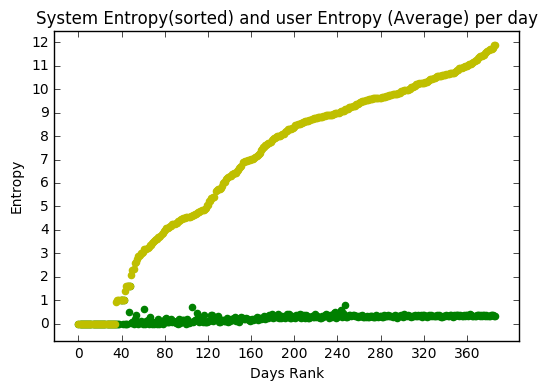
\includegraphics{entropy.png}
   \caption{Visualization of entropy}
     \label{fig:dig} 
\end{figure}


We can see that as the author mentioned, user's attention remains constant trough the days, contrary to the system's entropy which grows almost exponentially. We interpret this as "No matter how many new memes are there out there, users will only be able to manage on average the same amount of memes".
%-------------------------------------------------------------------------------

%-------------------------------------------------------------------------------

\section{Measuring inequality (10 points)}

We provide you with a sample implementation of the Chinese Restaurant Process\footnote{File ``chinese\_restaurant.py"; Additional information can be found here: \url{https://en.wikipedia.org/wiki/Chinese_restaurant_process}}.

Assume there is a restaurant with an infinite number of tables. 
When a new customer enters a restaurant he chooses an occupied table or the next empty table with some probabilities.


According to the process first customer always sits at the first table. 
Probability of the next customer to sit down at an occupied table $i$ equals 
 ratio of guests sitting at the table ($c_i/n$), where $n$ is the number of guests in the restaurant and $c_i$ is the number of guests sitting at table $i$.\\
 Probability of customer to choose an empty table equals :  $1- \sum_{i=1}^{S}{p_i}$, where $S$ is the number of occupied tables and ${p_i}$ = $c_i/n$.
 
Provided script simulates the process and returns number of people sitting at each table. We will study restaurants for 1000 customers.
Now you should modify the code and evaluate how unequal were the customers' choices of tables.   

%In this exercise,
%you should use it to simulate the growth of a network via the following process:
%\begin{itemize}
%\item A customer X sitting at a table Y, represents an edge from node X to node Y .
%\item With X tables occupied, a new customer taking a new table, will take place at table X + 1.
%\end{itemize}

% In the lecture `Herding Behavior' we discussed paper\footnote{`Experimental Study of Inequality and Unpredictability in an Artificial Cultural Market.', can be accessed from  \url{https://www.princeton.edu/~mjs3/salganik_dodds_watts06_full.pdf} } by Salganik et al. The authors used the Gini-coefficient to measure the inequality and in the lecture you have see how this coefficient stabilizes over time.

%Simulate a network with the Chinese Restaurant process and 
Calculate the Gini-
coefficient measuring the inequality between the tables,
until the coefficient stabilizes. Do five different runs and plot your results in a similar way that plots in the lecture slides are done, cf. Slide 32 and Slide 33.

\textbf{Answers:}
\begin{lstlisting}
import random
import numpy as np
import matplotlib.pyplot as plt
import matplotlib.patches as mpatches

def plot(ginis,restaurants):
    # The y values. Cumulative percentage of incomes
    j = 0
    for restaurant in restaurants:
        y, y_pe = [], []
        i = 0
        restaurant = sorted(restaurant)
        for rest in restaurant:
            prob = rest*100/sum(restaurant)
            if i == 0:
                y.append(prob)
            else:
                y.append(prob + y[i-1])
            i += 1

        # The perfect equality y values. Cumulative percentage of incomes.
        y_pe = np.linspace(0.0, 100.0, len(y))

        plt.title("Gini " + str(round(ginis[j],2)))
        plt.plot(y, label='lorenz', color='r')
        plt.plot(y_pe, label='perfect_equality', color='b')
        plt.ylabel('Percentage of guests')
        plt.xlabel('No. of tables')
        x_legend = mpatches.Patch(color='red', label='observations')
        y_legend = mpatches.Patch(color='blue', label='perfect equality')
        plt.legend(handles=[x_legend, y_legend], loc=5)
        plt.show()
        j += 1

def gini(restaurant):
    ordered = sorted(restaurant)
    height, area_under_curve = 0, 0
    for value in ordered:
        height += value
        area_under_curve += height - value / float(2)
    area_under_equity = height * len(restaurant) / float(2)
    gini = (area_under_equity - area_under_curve) / area_under_equity
    return gini


def generateChineseRestaurant(customers):
    # First customer always sits at the first table
    tables = [1]
    #for all other customers do
    for cust in range(2, customers+1):
            # rand between 0 and 1
            rand = random.random()
            # Total probability to sit at a table
            prob = 0
            # No table found yet
            table_found = False
            # Iterate over tables
            for table, guests in enumerate(tables):
                # calc probability for actual table an add it to total probability
                prob += guests / (cust)
                # If rand is smaller than the current total prob., customer will sit down at current table
                if rand < prob:
                    # incr. #customers for that table
                    tables[table] += 1
                    # customer has found table
                    table_found = True
                    # no more tables need to be iterated, break out for loop
                    break
            # If table iteration is over and no table was found, open new table
            if not table_found:
                tables.append(1)
    return tables
 
restaurants = 1000
network, ginis = [], []
for iterations in range(1, 6):
    network.append(generateChineseRestaurant(restaurants))
for net in network:
    ginis.append(gini(net))

plot(ginis,network)
\end{lstlisting}

\begin{figure}[h]
  \centering
  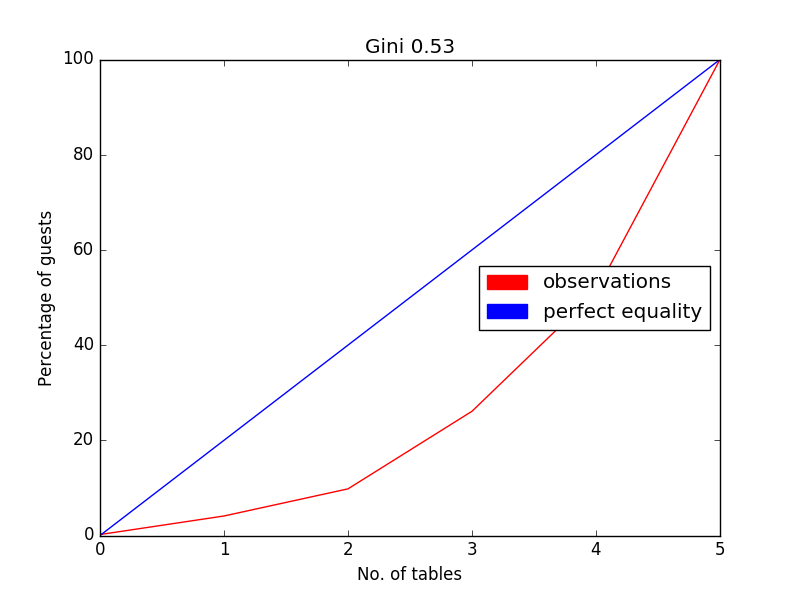
\includegraphics[scale = 0.5]{gini1.png}
   \caption{Gini Equality for the first iteration}
     \label{fig:dig} 
\end{figure}

\begin{figure}[h]
  \centering
  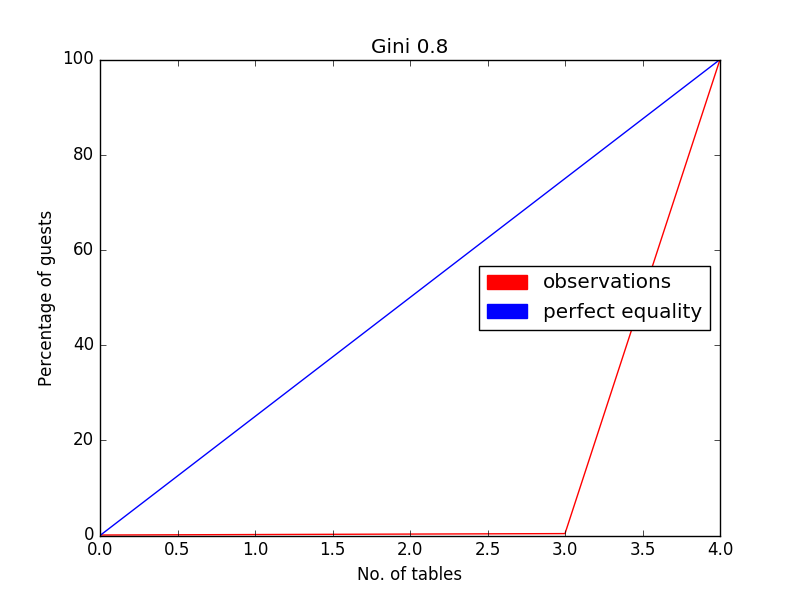
\includegraphics[scale = 0.5]{gini2.png}
   \caption{Gini Equality for the second iteration}
     \label{fig:dig} 
\end{figure}

\begin{figure}[h]
  \centering
  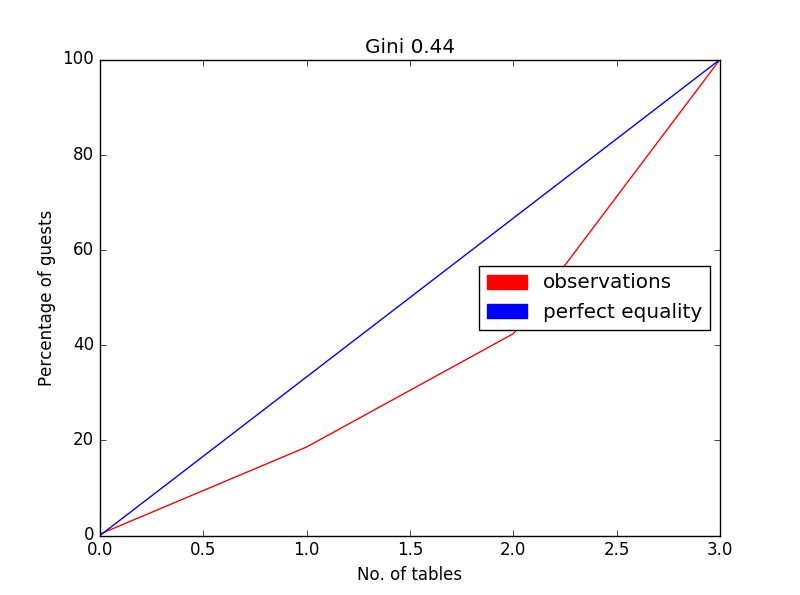
\includegraphics[scale = 0.5]{gini3.png}
   \caption{Gini Equality for the third iteration}
     \label{fig:dig} 
\end{figure}

\begin{figure}[h]
  \centering
  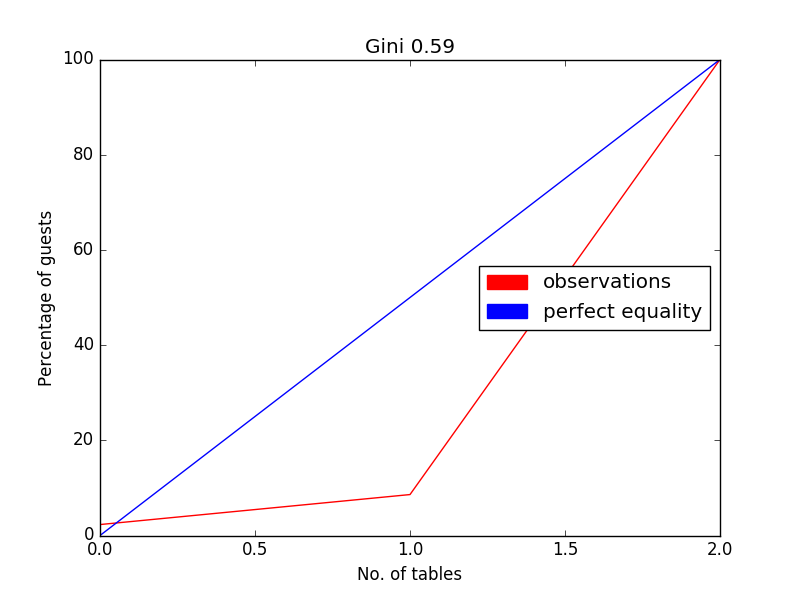
\includegraphics[scale = 0.5]{gini4.png}
   \caption{Gini Equality for the forth iteration}
     \label{fig:dig} 
\end{figure}

\begin{figure}[h]
  \centering
  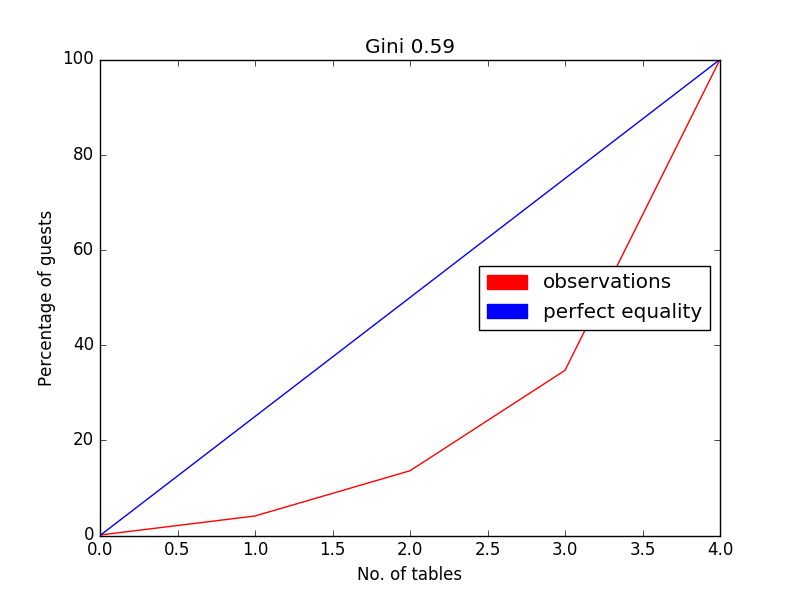
\includegraphics[scale = 0.5]{gini5.png}
   \caption{Gini Equality for the fifth iteration}
     \label{fig:dig} 
\end{figure}
%-------------------------------------------------------------------------------

%-------------------------------------------------------------------------------

\section{Herding (10 points)}
Let us consider the altitude of Koblenz to be 74 m above sea level. You are asked to figure out the height of the Ehrenbreitstein Fortress and the Fernmeldeturm Koblenz without googling.\\
The exercise is split in two parts:\\ \\
\underline{Part 1 : The Secret}\\
In \textit{complete secrecy}, each member of the team will write down their estimated height of the Ehrenbreitstein Fortress without any form of discussion. Please keep in mind that you need to have reasons for your assumption. Once you are done, then openly discuss in the group and present you values in a tabulated format with the reasons each one assumed to arrive at that value. 

\underline{Part II : The Discussion}\\
Discuss amongst yourself with valid reasoning  what could be the height of the Fernmeldeturm Koblenz. Only after discussing, each member of the group is asked to arrive at a value and present this value in a tabulated format as was done in Part I. \\ \\
Calculate the Mean, Standard Deviation and Variance of your noted results for both the cases and explain briefly what you infer from it. 

\textbf{Note:} This exercise is for you to understand the concepts of herding and not to get the perfect height by googling information. There is in fact no point associated with the height but with the complete reasoning that you provide for your answers. \\ \\

\begin{center}
\begin{tabular}{ | c | c | p{7cm} | }
\hline
Monument & Height (in meters) & Reasoning \\
\hline
 Fortress & 240 & The lenght of the seilbahn don't seem that long so the mountain can't be that tall \\ 
 \hline
 Fortress & 300 & Taking into consideration that Koblenz is at a 74 m altitude, as the fortress stands on small hill it can't be taller than estimated. \\  
 \hline
 Fortress & 375 & Compared to Deutsches Eck the hill seems tall enough for me to reach about this height.  \\
\hline
 Tower & 400 &  I just assume the tower is in a much higher hill than the fortress. Therefore i think is this much higher  \\
 \hline
 Tower & 450 & Based on my initial guess about the fortress. I believe that the tower is a copule of hundred meters taller than this hill altitude.  \\
 \hline
 Tower & 450 & I think this tower is located on a hill that is considerably much taller than the fortress.  \\
 \hline
\end{tabular}
\end{center}


\begin{figure}[h]
  \centering
  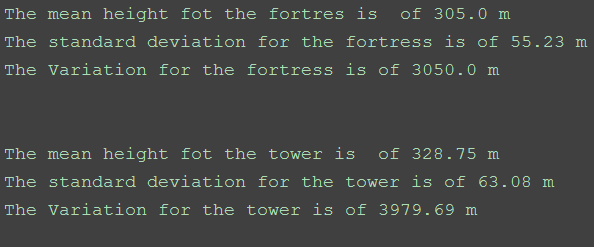
\includegraphics{guesses.png}
   \caption{Results}
     \label{fig:dig} 
\end{figure}




\makefooter

\end{document}
